\chapter{RESULTADOS E DISCUSSÕES}

Os resultados obtidos, a partir do desenvolvimento de  6 sistemas de misturas binárias, foram subdivididos em subitens nos estudos de casos. Esses estudos contemplam misturas de ácidos graxos e álcoois, sendo a aplicação da modelagem matemática utilizada inovadora neste último grupamento funcional.

Para comparar os resultados obtidos,  gráficos foram construídos, gerando diagramas de fases sólido-líquido, evidenciados pelas características mais relevantes: linha \textit{liquidus}, ponto eutético e/ou ponto peritético, a partir da aplicação dos  modelos MA, MS e Wilson, já descritos anteriormente.

A escala de cada diagrama de fase das misturas binárias são distintas, pelo fato de que cada ácido graxo ou álcool possui ponto de fusão distintos como podemos verificar nas seções \ref{sec:1} até \ref{sec:6}.

A partir dos dados experimentais coletados do referencial teórico utilizado determinados pela técnica de DSC, o DSC é uma técnica com a finalidade de encontrar os limites de fase, a partir de medidas dos efeitos térmicos durante o processo de mudança de fase.

A metodologia estatística de $R^2$ (coeficiente de determinação) foi aplicada, para determinar o percentual em que a metodologia de DSC está representada pelo algoritmo, com os modelos MA, MS e \textit{Wilson}.

\section{Estudos de casos.}

\subsection{Sistema 1: Ácido Mirístico e Ácido Esteárico}\label{sistema1}
Com a aplicação da modelagem matemática na seção \ref{subsection:1}, cujo desenvolvimento resultou em um modelo de PNL, foi possível obter o diagrama de fase sólido-líquido para esse sistema.

Na Figura \ref{fig:3} o diagrama de fase foi determinado pelos modelos termodinâmicos \textit{MA}, \textit{MS} e \textit{Wilson} implementado no \textit{GAMS} e o gráfico gerado pelo \textit{PyCharm} com biblioteca do \textit{R}. Os dados experimentais comparativos foram obtidos por COSTA 2009 por experimentos com o método de DSC.
\begin{figure}[H]
	\centering
	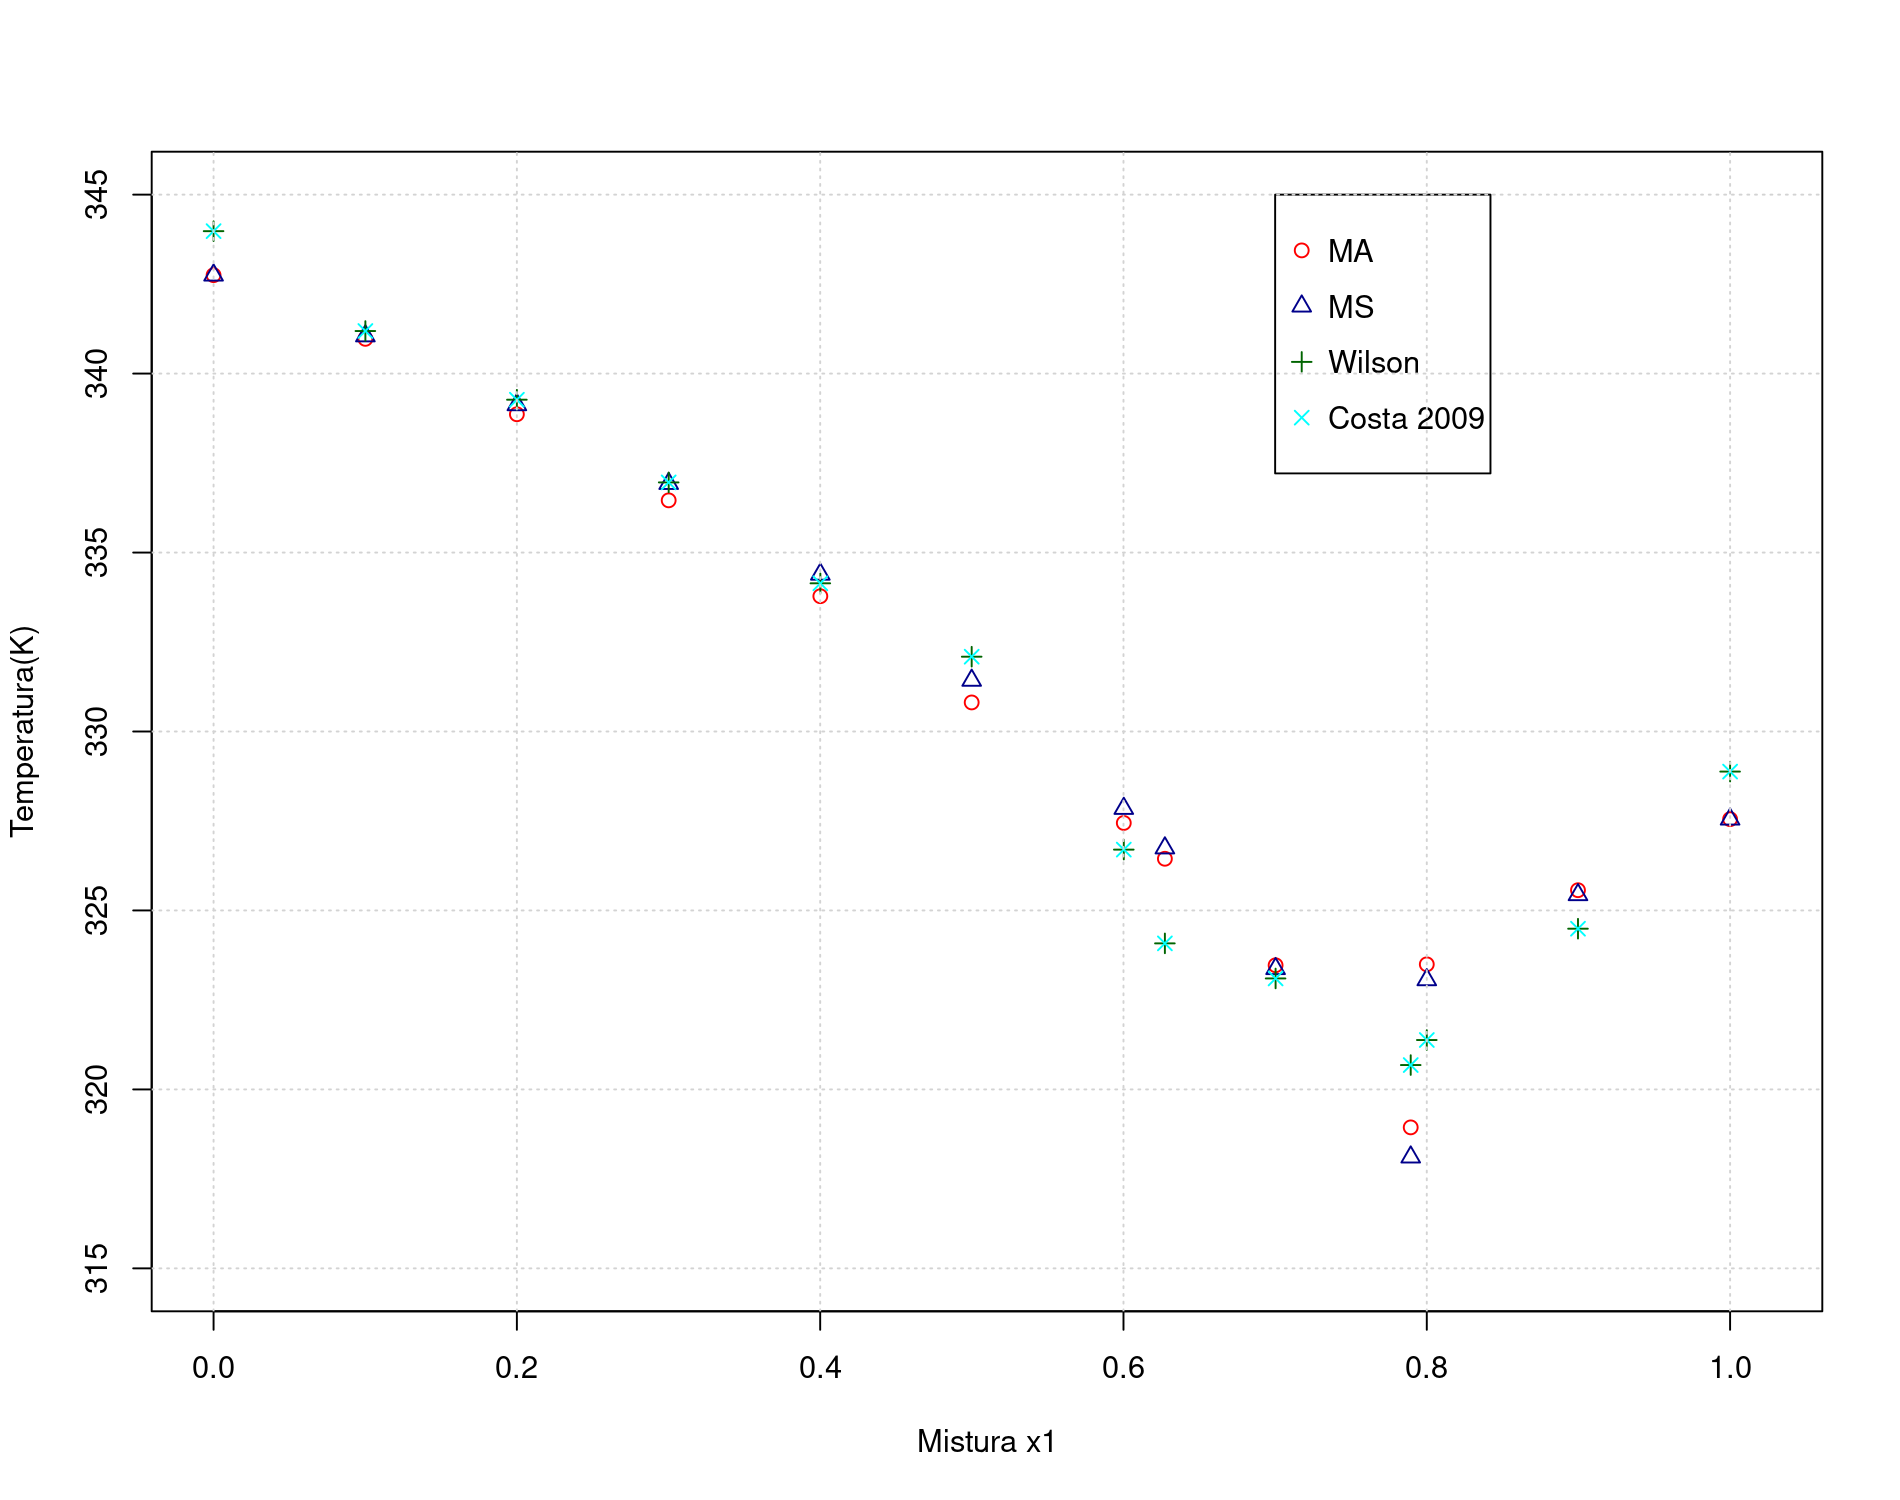
\includegraphics[width=1.06\linewidth 
	%,height=0.4\textheight
	]{dados/figuras/Miristico_estearico.png}
	\caption[Diagrama do equilíbrio sólido-líquido para mistura Ácido Mirístico e Ácido Esteárico]{Diagrama do equilíbrio sólido-líquido para mistura Ácido Mirístico(1) e Ácido Esteárico(2) (\textit{PyCharm}/$R$)}
	\label{fig:3}
\end{figure}

A partir do diagrama de fases obtido, evidencia-se a formação da linha \textit{liquidus} praticamente sobreposta aos dados experimentais comparativos, e entre os modelos termodinâmicos estudados, até a composição aproximada de 50\% da mistura ácido mirístico e ácido palmítico. Após essa medida intermediária, verifica-se maior distanciamento das técnicas computacionais aplicadas, comparada ao dados de DSC, porém mantém-se a inclinação desejada, com a percepção da formação do ponto eutético próximo a composição 0,6 e uma outra visualização de mudança de inclinação próximo a composição 0,8, referindo-se a presença do ponto peritético. Vale ressaltar a relevância teórico/computacional da sensibilidade e robustez de modelos termodinâmicos serem capazes de prever tais pontos específicos de transição, principalmente o ponto peritético.

%\begin{comment}
%\subsection{Sistema 2: Ácido Palmítico e Ácido Esteárico} \label{sistema2}
%Aqui também a aplicação da modelagem matemática já citada, cujo desenvolvimento resultou em um modelo de \textit{PNL}, foi possível obter o diagrama de fase sólido-líquido para esse sistema.
%Na Figura \ref{fig:4} o diagrama de fase foi determinado pelos modelos termodinâmicos \textit{MA}, \textit{MS} e \textit{Wilson} implementado no \textit{GAMS} e o gráfico gerado pelo \textit{PyCharm} com biblioteca do \textit{R}.
%\begin{figure}[H]
%	\centering
%	\includegraphics[width=1.06\linewidth 
	%,height=0.4\textheight
%	]{dados/figuras/Palmitico_estearico_DSC.png}
%	\caption[Diagrama do equilíbrio sólido-líquido para mistura Ácido Palmítico e Ácido Esteárico]{Diagrama do equilíbrio sólido-líquido para mistura Ácido Palmítico(1) e Ácido Esteárico(2) (\textit{PyCharm}/\textit{R}) Autor.}
%	\label{fig:4}
%\end{figure}
%\end{comment}


\subsection{Sistema 2: Ácido Palmítico e Ácido Esteárico}\label{sistema3}



Com a definição dos pares ordenados para composição de mistura e temperatura,  foi possível obter a linha \textit{liquidus} praticamente sobreposta aos dados experimentais comparativos próximos as composições de substância pura, em que visualmente o modelo de Margules Assimétrico tem maior proximidade aos dados experimentais. Quanto a inclinação das curvas definidas pelas regiões calculadas, são apresentadas inclinações equivalentes aos dados experimentais.  Ressalta-se a importância de modelos teórico/computacionais apresentarem, pela aplicação dos modelos termodinâmicos adequados, a capacidade de predição de formação do ponto eutético.




\section{Coeficiente de Determinação}

O Coeficiente de Determinação ou $R^2$ foi aplicado como técnica comparativa entre os resultados obtidos da literatura ao utilizar experimentalmente a técnica de DSC (Calorimetria exploratória diferencial) aos modelos MA, MS e Wilson em cada um dos sistemas, para averiguação da representatividade de cada modelo. Dessa forma considerados os dados de DSC como $VD$ (variável dependente) ou variável resposta e dos modelos aplicados como $VI$ (variável independente) ou variável de regressão. O $R^2$ fornece um valor em percentagem ou valor decimal cuja a interpretação é, quantos de $VD$ é explicada por $VI$ ou quantos que $VI$ tem influencia sobre $VD$, isto é, $R^2$ é a proporção da variação de $VD$ explicada pela variação de $VI$. 

A propriedade do coeficiente de determinação é que:
\begin{itemize}
    \item $R^2\in [0;1]$
    \item $R^2=1$, $VD$ é explicada pela variação de $VI$ em 100\%
    \item $R^2=0$, $VI$ não tem influencia sobre $VD$.
\end{itemize}

O valor do $R^2$ é calculado pela fórmula
\begin{equation}
    R^2=\frac{\left(\displaystyle\sum_{i=1}^{n}x_i\cdot y_i-n\cdot\overline{x}\cdot\overline{y}\right)^2}{\left(\displaystyle\sum_{i=1}^{n}x_i^2-n\cdot\overline{x}^2\right)\times\left(\displaystyle\sum_{i=1}^{n}y_i^2-n\cdot\overline{y}^2\right)}
\end{equation}
em que $n$ quantidade de elementos da variável $VD$ ou $VI$, $x_i\in VI$ e $y_i\in VD$.
\begin{equation}
    \overline{x}=\frac{\displaystyle\sum_{i=1}^{n}x_i}{n}
\end{equation}
e
\begin{equation}
    \overline{y}=\frac{\displaystyle\sum_{i=1}^{n}y_i}{n}
\end{equation}

%\begin{center}
    %Coeficiente de determinação da variável dependente  técnicas de %DSC e variáveis independentes MA, MS ou Wilson
%\end{center}
\begin{table}[H]
    \caption{Coeficiente de Determinação}
    \centering
    \begin{tabular}{l|p{3cm}p{3cm}p{3cm}}
    %\multicolumn{4}{c}{\textbf{Coeficiente de determinação da variável dependente  técnicas de DSC e variáveis}}  \\ 
    %\multicolumn{4}{c}{\textbf{independentes MA, MS ou Wilson}} \\ 
    \hline
         & $R^2$ MA & $R^2$ MS & $R^2$ Wilson \\
    \hline
    Ac. Mirístico e Ac. Esteárico  & 0.9756  & 0.9706 & 0.9708 \\
    Ac. Palmítico e Ac. Esteárico  & 0.9699  & 0.8005 & 0.7040 \\
    %Ac. Palmítico e Ac. Esteárico  & 0.4955  & 0.5355 & 0.5057 \\
    Hexadecanol e Ac. Mirístico  & 0.2427  & 0.2328 & 0.2133 \\
    Hexadecanol e Tetradecanol  & 0.9804  & 0.9310 & 0.9887 \\
    Ac. Esteárico e Ac. Linoleico  & 0.1483  & 0.5592 & 0.8745 \\
    Ac. Palmítico e Ac. Linoleico  & 0.7490  & 0.5602 & 0.0000 \\
    \end{tabular}
    \label{tab:1}
\end{table}

